\documentclass[10pt,a4paper,oneside]{article}
\usepackage{cmap}
\usepackage[T2A]{fontenc}
\usepackage{float}
\usepackage{listings}
\usepackage{csquotes}
\usepackage[utf8]{inputenc}
\usepackage{amsmath}
\usepackage{amsfonts}
\usepackage{amssymb}
\usepackage[english, russian]{babel}%Подключаем русский язык.
\usepackage{graphicx}
\usepackage{geometry} % Меняем поля страницы.
\geometry{left=3cm} %Левое поле.
\geometry{right=2cm} %Правое поле.
\geometry{top=3cm} %Верхнее поле.
\geometry{bottom=2cm} %Нижнее поле.


%Начало документа
\begin{document}

%Создаём титульник.
\begin{titlepage}
\newpage
	%Название ВУЗа и институт.
	\begin{center}
		\Large Санкт-Петербургский Государственный Политехнический Университет\\
		Институт Компьютерных Наук и Технологий\\
	\end{center}
	%Кафедра.
	\begin{center}
		\large\textbf {Высшая школа интеллектуальных систем и суперкомпьютерных технологий}
	\end{center}
	
	%Пропуск места. 
	\vspace{5em}
	%!!!!!!!!!!!!!!!!!!!!!!!!!!!!!!!!!Название работы.
	\begin{center}
		\large{Отчёт по лабораторной работе №10 \\ на тему \\
		\textbf{Линейный стационарные системы} }
	\end{center}
	
	%Делаем пропуск и пишем студента и преподавателя.
	\vspace{25em}
	\begin{flushright}
		\textbf{Работу выполнил\\}Студент группы 3530901/80203 \\ Танашкин В.А.\\
		\textbf{Преподаватель\\}Богач Н.В. 
	\end{flushright}
	
	\vspace{\fill}%В самом низу
	\begin{center}
	Санкт-Петербург, 2021 год	
	\end{center}
\end{titlepage} %Закончили титульный лист.

\section{Настройка проекта}
Перед тем как выполнять задания необходимо настроить проект и сделать все необходимые импорты:

\begin{figure}[H]
        \centering
        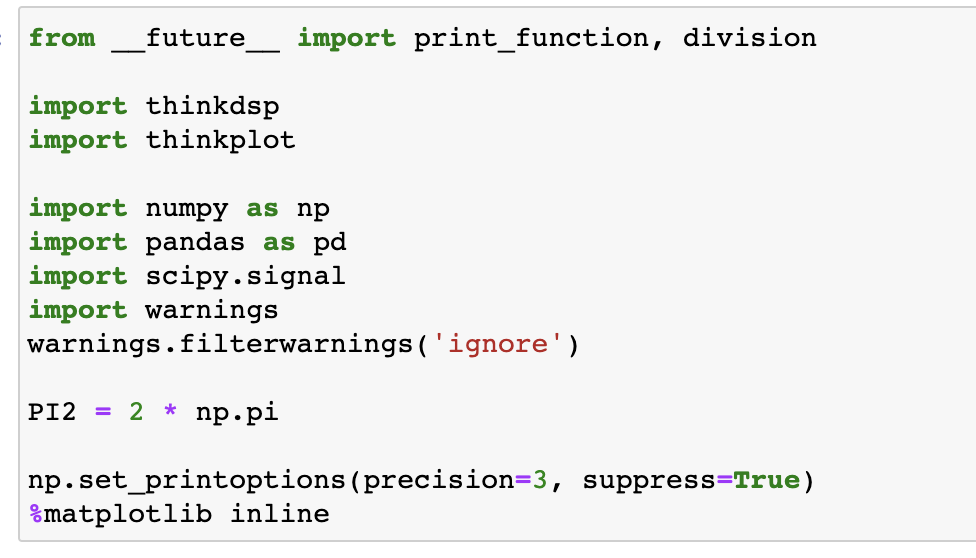
\includegraphics[width=0.75\textwidth]{pics/0.png}
        \caption{2}
        \label{fig:first}
\end{figure}

\section{Упражнение номер №1}

Убедиться что дополнение нулями устраняет лишнюю ноту в начале фрагмента

Я усекаю оба сигнала до 2^16 элементов, а затем обнуляю их до 2^17. Использование степени двойки делает алгоритм DFT наиболее эффективным.

Вот импульсный отклик:

\begin{figure}[H]
        \centering
        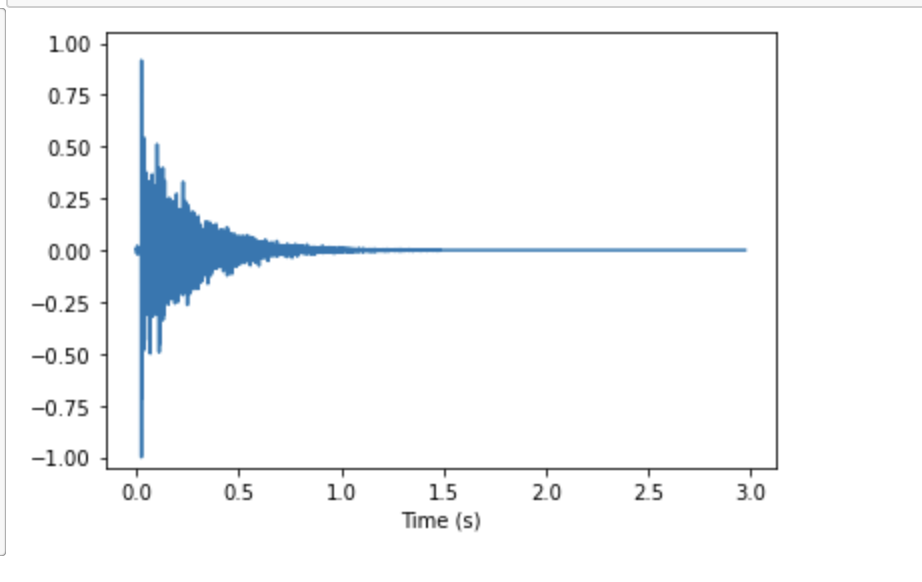
\includegraphics[width=0.75\textwidth]{pics/1.png}
        \caption{2}
        \label{fig:first}
\end{figure}

Выведем спектр:

\begin{figure}[H]
        \centering
        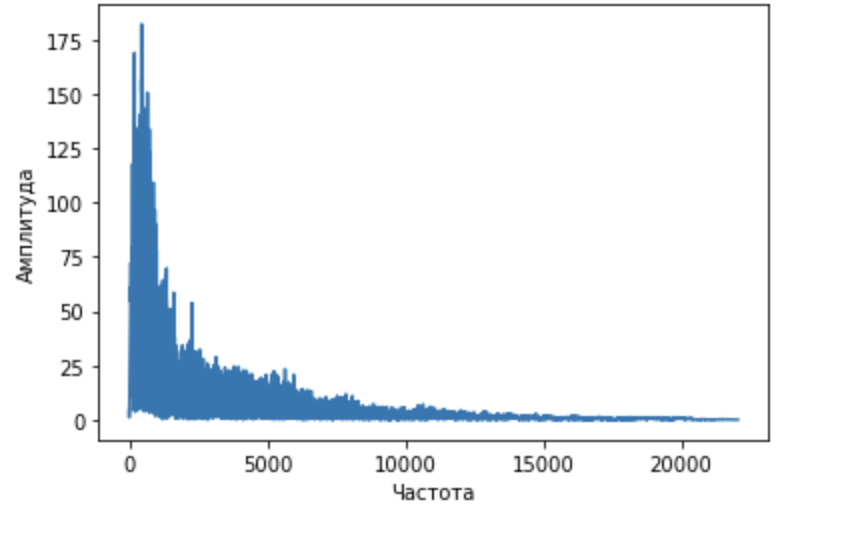
\includegraphics[width=0.75\textwidth]{pics/2.png}
        \caption{2}
        \label{fig:first}
\end{figure}

Рассмотрим еще один сигнал:

\begin{figure}[H]
        \centering
        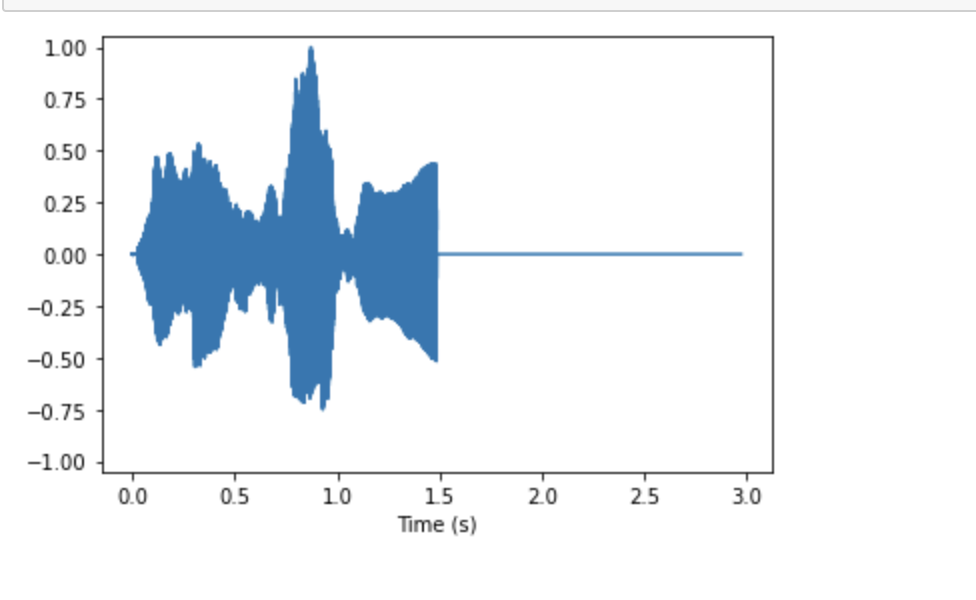
\includegraphics[width=0.75\textwidth]{pics/3.png}
        \caption{2}
        \label{fig:first}
\end{figure}

Теперь умножим DFT сигнала на передаточную функцию и преобразуем обратно в волну:

\begin{figure}[H]
        \centering
        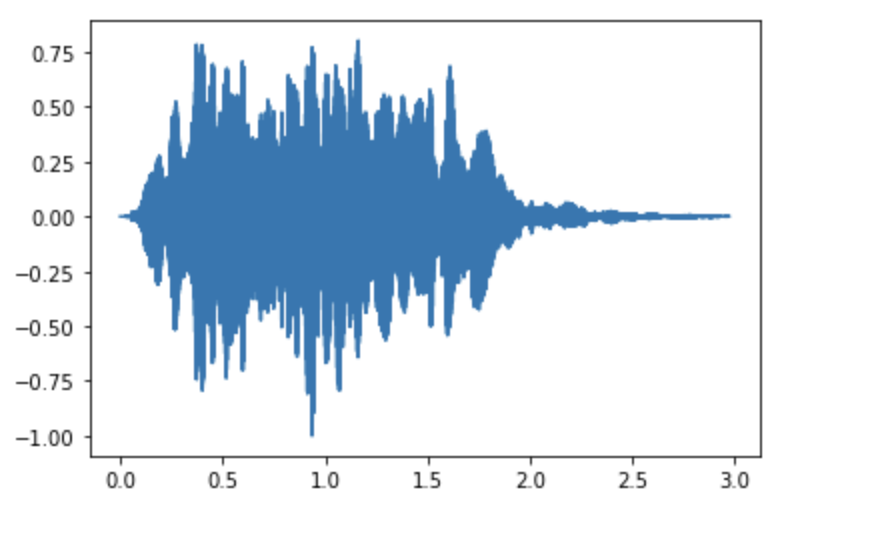
\includegraphics[width=0.75\textwidth]{pics/4.png}
        \caption{2}
        \label{fig:first}
\end{figure}

Результат не выглядит так, как будто он оборачивается вокруг:

Мы должны получить такие же результаты от np.convolve и scipy.signal.fftconvolve.

Обрежем нулевой отступ:

\begin{figure}[H]
        \centering
        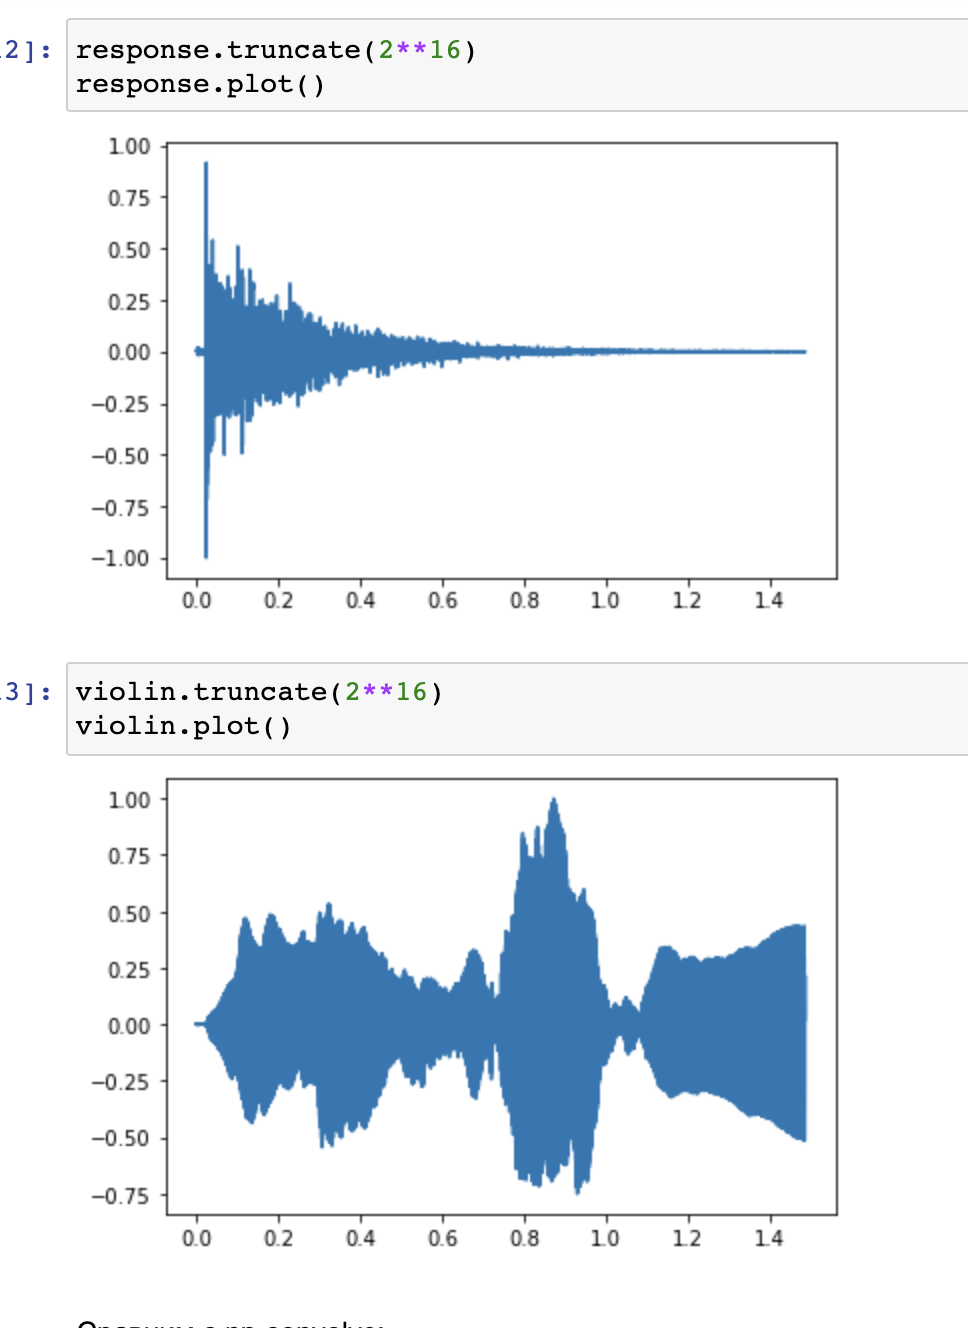
\includegraphics[width=0.75\textwidth]{pics/5.png}
        \caption{2}
        \label{fig:first}
\end{figure}

Сравним с np.convolve:

\begin{figure}[H]
        \centering
        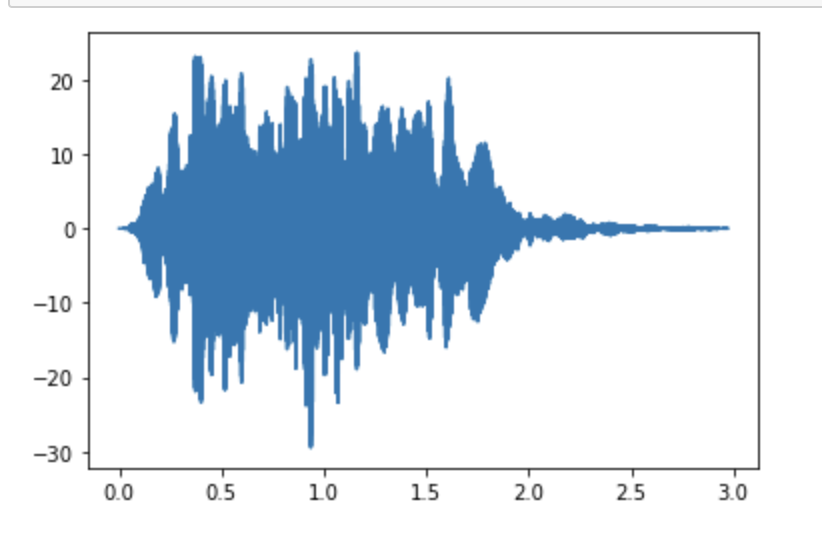
\includegraphics[width=0.75\textwidth]{pics/6.png}
        \caption{2}
        \label{fig:first}
\end{figure}

Как мы можем наблюдать результаты очень похожи.

\begin{figure}[H]
        \centering
        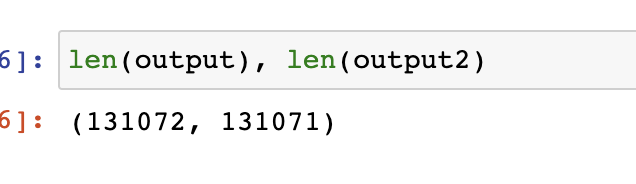
\includegraphics[width=0.75\textwidth]{pics/7.png}
        \caption{2}
        \label{fig:first}
\end{figure}

Но результаты не совсем одинаковой длины.

scipy.signal.fftconvolve делает то же самое, но, как следует из названия, он использует DFT, поэтому он значительно быстрее:

\begin{figure}[H]
        \centering
        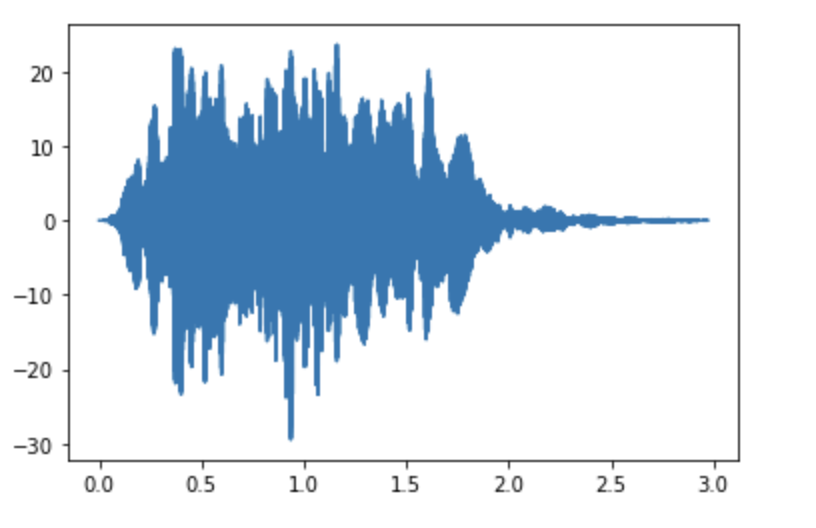
\includegraphics[width=0.75\textwidth]{pics/8.png}
        \caption{2}
        \label{fig:first}
\end{figure}

Результат такой же.

\section{Упражнение номер №2}

Необходимо смоделировать двумя способами в том пространстве где была измерена импульсная характеристика.

Возьмем звук из репозитория: 

\begin{figure}[H]
        \centering
        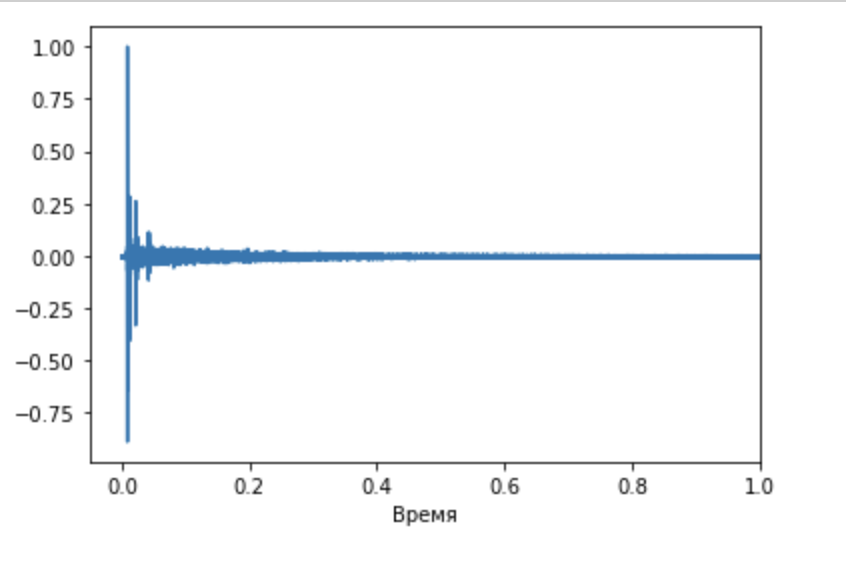
\includegraphics[width=0.75\textwidth]{pics/9.png}
        \caption{2}
        \label{fig:first}
\end{figure}

DFT импульсной характеристики - это передаточная функция:

\begin{figure}[H]
        \centering
        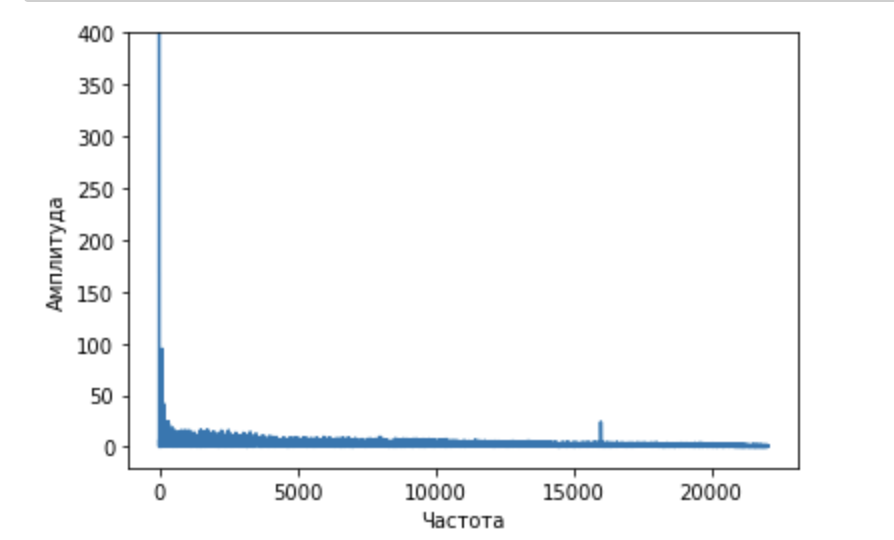
\includegraphics[width=0.75\textwidth]{pics/10.png}
        \caption{2}
        \label{fig:first}
\end{figure}

Рассмотрим график в логарифмической метрики:

\begin{figure}[H]
        \centering
        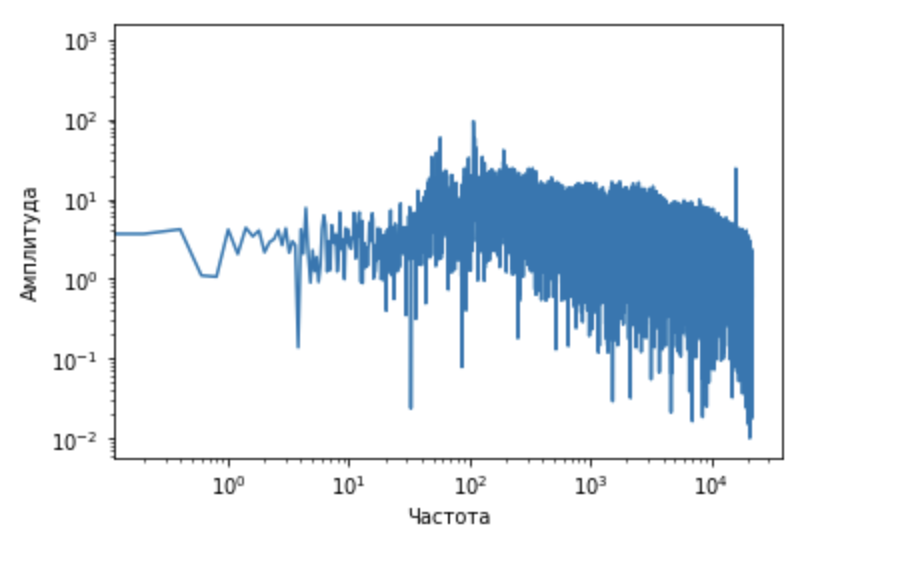
\includegraphics[width=0.75\textwidth]{pics/11.png}
        \caption{2}
        \label{fig:first}
\end{figure}

Теперь мы можем смоделировать звучание записи, если бы ее воспроизвели в одной комнате и записали бы таким же образом.

Возьмем еще одну запись из репозитория:

\begin{figure}[H]
        \centering
        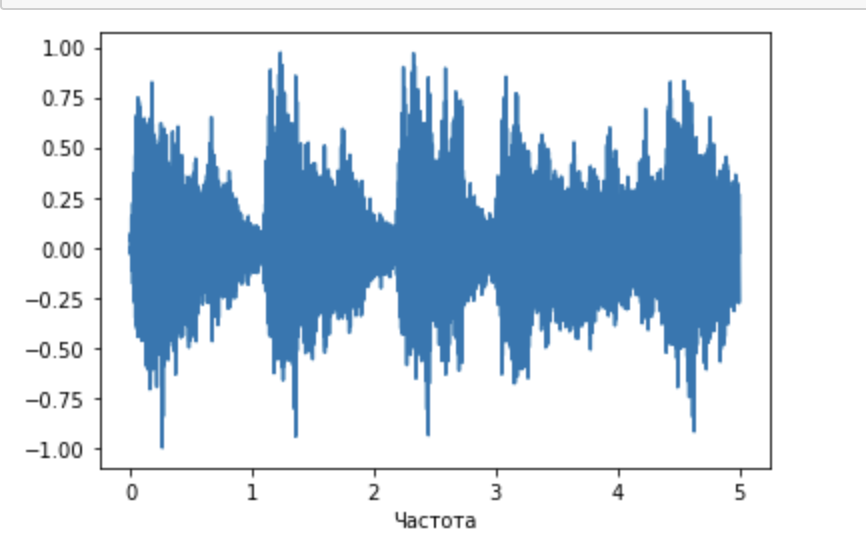
\includegraphics[width=0.75\textwidth]{pics/12.png}
        \caption{2}
        \label{fig:first}
\end{figure}

Теперь мы вычисляем DFT записи скрипки. Обрежем запись скрипки до той же длины, что и импульсная характеристика:

\begin{figure}[H]
        \centering
        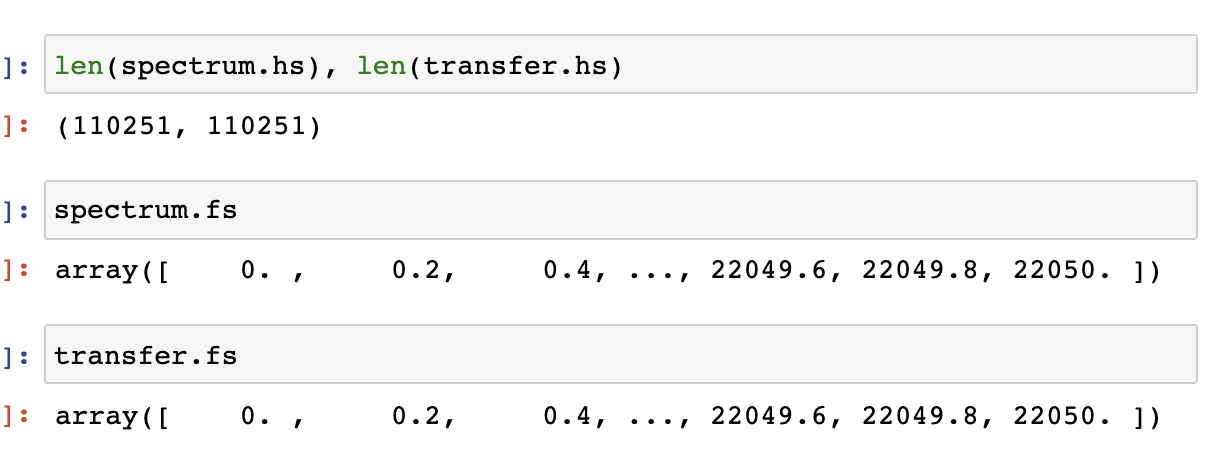
\includegraphics[width=0.75\textwidth]{pics/13.png}
        \caption{2}
        \label{fig:first}
\end{figure}

Теперь мы можем умножить в частотной области и преобразовать обратно во временную область. Проведем сравнение:

\begin{figure}[H]
        \centering
        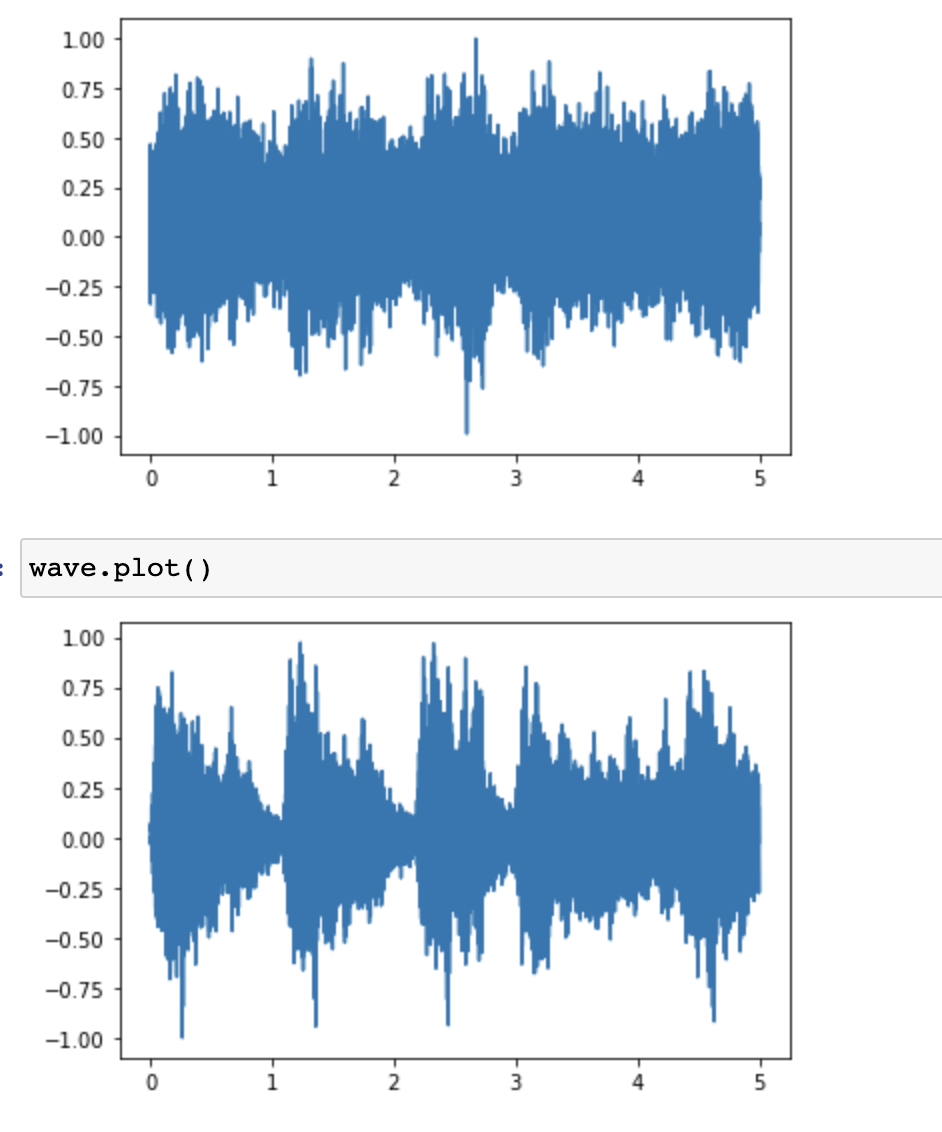
\includegraphics[width=0.75\textwidth]{pics/14.png}
        \caption{2}
        \label{fig:first}
\end{figure}

Теперь, когда мы распознаем эту операцию как свертку, мы можем вычислить ее с помощью метода convolve


\end{document}
